\chapter{Introduction}\label{introduction} %1000 words

A conventional Electric power system comprises of a generator, transmission system, distribution system and end consumers. Initially, they were localised and often the consumer was directly connected to the generator. However, as the complexity and scale of consumers increases the demand for centralised systems was born where multiple consumers were connected to the same generator using transmission and distribution networks. Later electricity demand patterns were identified which led to improvements in the power grids. They had extra generators to manage peak loads while the other generators ran full-time. As technology progressed more methods were made possible for power generation including Photo Voltaic cells which people installed in their homes at subsidized rates. This led to an imbalance where power generation was no longer limited to power plants and the grids had to modernise to accept power back from the consumers to prevent wastage.

\begin{figure}[h]
    \centering
    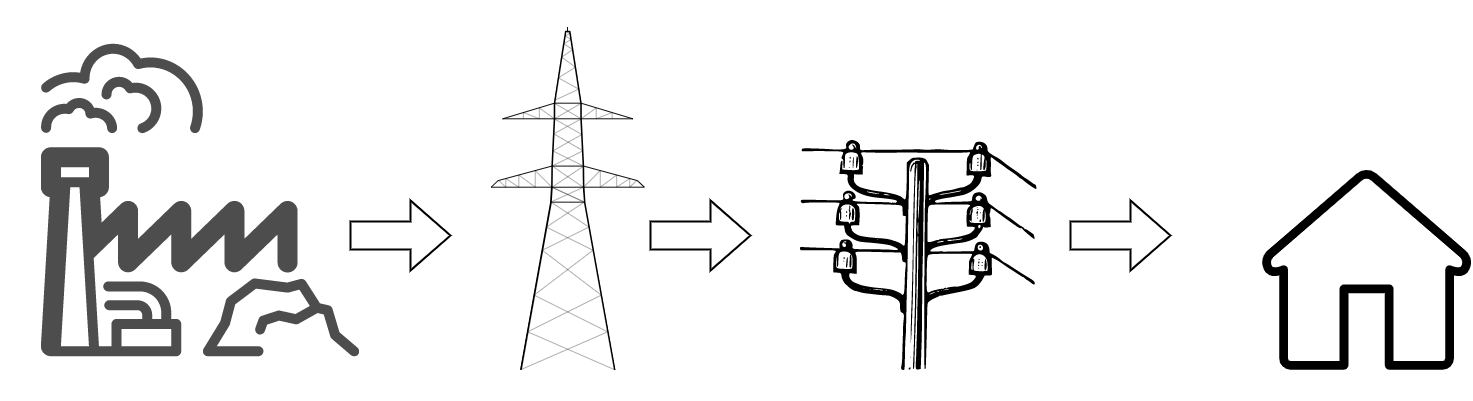
\includegraphics[width=0.8\textwidth]{ElectricalGrid.png}
    \caption{A typical electrical grid}
    \label{fig:ElectricalGrid}
\end{figure}

Smart grids are known to be the future of electricity distribution with a bi-directional flow of information and power to form an advanced automated energy delivery network \citep{RN6}. The main features of a smart grid are clean, safe, secure, reliable, resilient, efficient, and sustainable[1]. IoT can serve as a means to connect different parts of the energy network and enable information flow. This information can then be used to monitor the system behaviour and various algorithms can be used to improve efficiency of the grid and also resulting in reduced environmental impact [2-4].

Over years various technologies have been examined for routing of data packets in smart grid networks [4-7]. Zeinali et al[8] says the best way to handle information for smart grids would be to utilize the already existing internet infrastructure. In the recent year internet technology has advanced significantly, now enabling internet access to every device using wireless technology. One such technology is LPWAN or Low-Power-Wide-Area-Networks [9]. Yuke Li examines the a licenced LPWAN technology name NB-IoT for its suitability to smart grids [10]. While Shalli et al[6] and Faheem et al[5] examined the suitability of routing protocols DCRN-GA and EQRP for routing of data in smart grids. This paper will build upon their work to compare the two protocols over an NB-IoT based network in the locality of Wollongong, NSW, Australia.
